% !TEX root = ../main.tex

\chapter{The SBN program at Fermilab and the ICARUS experiment}
\label{chap:icarus_detector}

%% BRIEF INTRODUCTION
The Short Baseline Neutrino experimental program at Fermi National Accelerator Laboratories aims to  draw a complete and consistent picture of the sterile neutrino scenario, depicted in detail in \autoref{chap:theory_introduction}. This is planned to be achieved by employing the Liquid Argon Time Projection Chamber technology with multiple functionally identical detectors on the same baseline at different positions with respect to the neutrino beam source. 

Albeit the original plan for a three-detector program, MicroBooNE finished its data-taking period in 2020, two years prior to ICARUS starting its data collection campaign and five prior to SBND, so the SBN program will perform a search for the sterile neutrino using a two-detector experiment, 

\section{The Short Baseline Neutrino program at Fermilab}

\subsection{Neutrino beam}

\paragraph{Booster Neutrino Beam}

\paragraph{Neutrinos at the Main Injector off-axis beam}

\subsection{Liquid Argon Time Projection Chambers}

\subsection{The SBN near detector: SBND}

\section{The ICARUS-T600 detector}

\begin{sidewaysfigure}
    \centering
    \begin{tikzpicture}
        \node at (0,0) {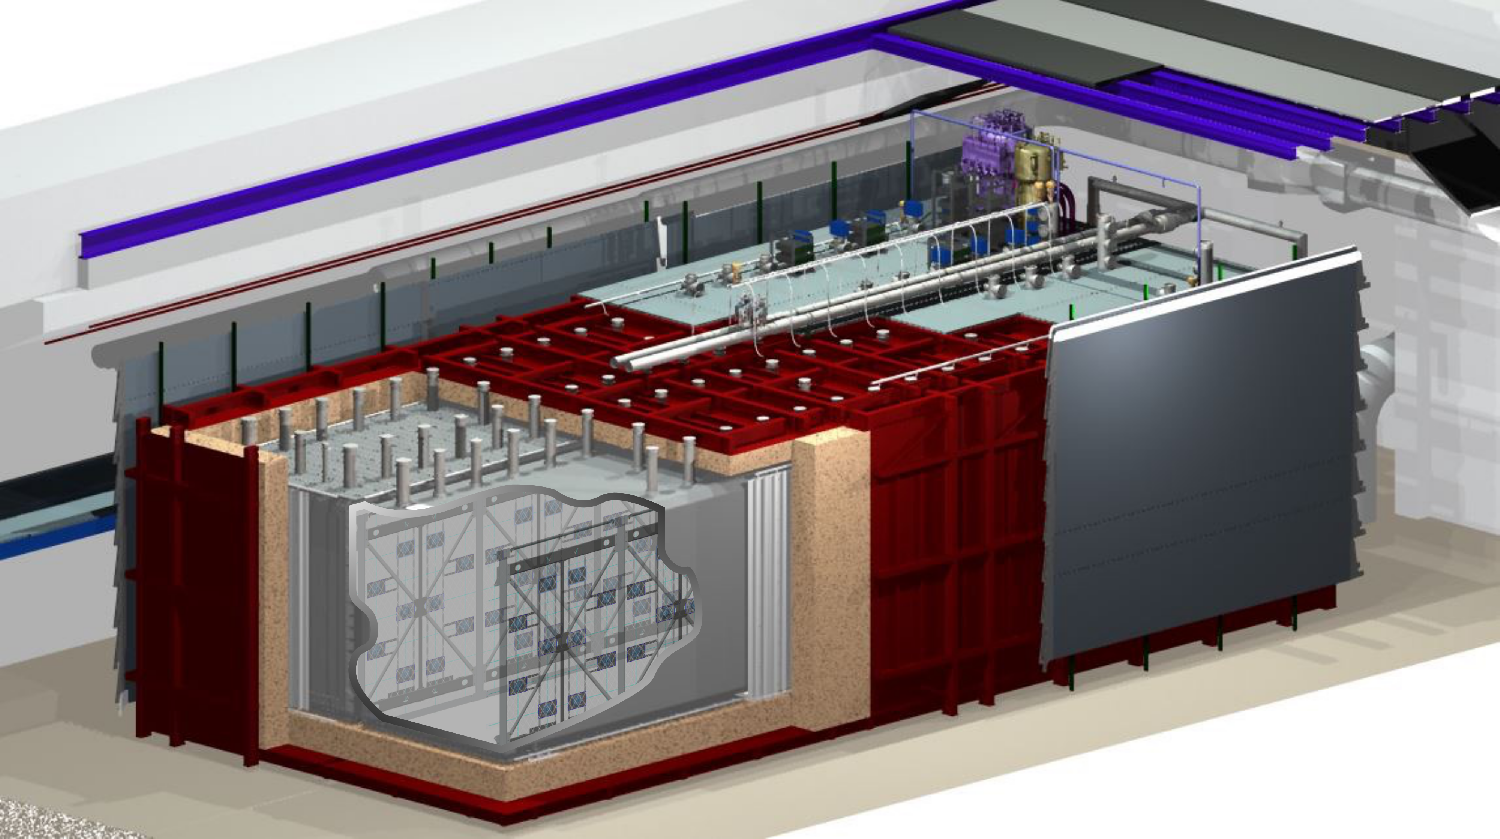
\includegraphics[width=\linewidth]{detector/SBN-FD_composite}};

        \draw[-*, white] (-1,2.5) node [left, white, fill=Gray!15!black] {TPC electronics} -- (0.5,2.25);
        \draw[-*, white] (-9,.5) node [right, white, fill=BrickRed] {Warm vessel} -- (-7.25,-1.5);
        \draw[-*, white] (4,2) node [right, white, fill=Plum!50!black] {Cryogenics} -- (3.25,3.5);
        \draw[-*, white] (7,-0.5) node [below, white, fill=Gray!15!black] {Top-CRT} -- (6.5,4);
        \draw[-*, white] (6,-1.75) node [right, white, fill=Gray!15!black] {Side-CRT} -- (5,-1);
        \draw[-*, white] (6,-3) node [above, white, fill=Gray!15!black] {Bottom-CRT} -- (3.5,-3.75);

        \draw[-*, white] (0,-4.5) node [below, white, fill=Gray!25!black] {East T300 cryostat} -- (-1,-3.5);
        \draw[-*, white] (-4.5,-4.5) node [left, white] {
            \begin{minipage}{4cm}
                \raggedleft
                TPC wireplanes + PMTs
            \end{minipage}} -- (-2.5,-2.5);

        \draw[-Latex, white] (-7,-3.5) -- (-7, -2.5) node[above] {$y$};
        \draw[-Latex, white] (-7,-3.5) -- (-6, -3.2) node[right] {$z$ (beam)};
        \draw[-Latex, white] (-7,-3.5) -- (-7.5, -3.35) node[left] {(drift) $x$};

        \draw[-*, black] (-4.5,5) node [left, black] {\SI{3}{m} concrete overburden} -- (-3,4.5);

        % \draw[step=1.0,white,thin] (-10,-5.5) grid (10,5.5);
        % \foreach \i in {-10,...,10} {
        %     \node [below] at (\i,-5.5) {$\i$};
        % }
        % \foreach \i in {-5,...,5} {
        %     \node [left] at (-10,\i) {$\i$};
        % }

        
    \end{tikzpicture}
    \caption[ICARUS detector illustration]{Illustration of the ICARUS T600 detector at Fermilab. Surrounding the warm vessel is the $4\pi$ coverage CRT. Above the warm vessel, the TPC readout warm electronics are placed, alongside the proximity cryogenics. Inside the warm vessel two identical (east and west) T300 modules are hosted, each containing two TPCs sharing a common cathode at the centre and two anode plane assemblies, one on each side.}
    \label{fig:ICARUS_scheme}
\end{sidewaysfigure}

\subsection{The ICARUS subsystems}

\paragraph{TPC}

\paragraph{Light collection system}

\paragraph{Cosmic ray tagger}


% Firstly proposed by Nobel laureate Carlo Rubbia \cite{Rubbia:1977zz}, the concept of Liquid Argon Time Projection Chambers (LArTPCs for short) was implemented in the Gran Sasso National Laboratories (LNGS) near L'Aquila (Italy) in the ICARUS (Imaging Cosmic And Rare Underground Signals) detector \cite{Bettini:1991fh, Cennini:1994pk, Cennini:1995tt, ICARUS:1995nrd}, which collected data between 2006 and 2011 \cite{Rubbia:2011ft}, alongside the OPERA, LVD and BOREXINO detectors from the CERN Neutrinos to Gran Sasso (CNGS) neutrino beam \cite{Kodama:2004db}. The main detectors for this project were the OPERA and ICARUS experiments, and were therefore called respectively CNGS1 and CNGS2.

% Today, the ICARUS T600 detector is one of the longest running LArTPC in existence. 

% After the results of the CNGS analysis were published the ICARUS detector moved in 2018 from LNGS, to the CERN facility, where it underwent a series of upgrades, both for electronics and in the liquid Argon purification system; serious upgrades were also performed on the exterior of the experiment where a cosmic ray tagger module was added; in 2020 the detector arrived to its current location in the SBN facility at Fermilab, where it has been detecting neutrinos since: mainly $\PGnGm$ and some $\PGne$s, from the Booster Neutrino Beam (BNB, on axis with the $z$ direction of the detector frame of reference) and from the Neutrino Main Injector (NuMI). 

% At the Short Baseline Neutrino (SBN) facility, the ICARUS experiment started its data run taking period in 2022 and has since ran thrice \cite{ICARUS:2023gpo}, with the latest data expected to be ready for the end of 2024 for the official analysis. Its younger brother, the SBND (Short Baseline Near Detector) experiment, finished the cryostat commissioning with some delays in 2023 and is now completing the commissioning of the cosmic ray tagger (CRT) modules, with the analysis on veto efficiency for the top CRT modules ongoing. 

% Joint efforts of the SBND and ICARUS detectors in the SBN collaboration will provide a highly efficient identification of neutrino interactions, strongly mitigating the possible sources of background and reducing the impact of systematics. 

% The combination of two nearly identical detectors allows for the measurement of neutrino oscillations over the distance in between the experiments, comparing the $\nu$s flux at \SI{110}{\meter} (SBND) and at \SI{600}{\meter} (ICARUS). 

% A third and a fourth experiment were also active in the BNB baseline, MiniBooNE (\mboone) and MicroBooNE (\uboone). The former completed its data taking period in 2018, and the latter was active between 2015 and 2021. Those two experiments provided strong ($\sim5\sigma$) evidence of event excess \cite{MiniBooNE:2018esg} in respect to what was expected (see figure \ref{fig:miniboone_results}). The main goal of the SBN collaboration is therefore to test this anomaly using data from BNB neutrinos. 

% In addition to this anomaly, ICARUS will also test the oscillation signal reported by the Neutrino-4 collaboration, hinting towards $\Delta m^2 \simeq \SI{7.26}{\electronvolt\squared}$ and $\sin^22\theta = 0.38$ ($3.5\sigma$ CL), both in $\PGne$ and $\PGnGm$ channels from BNB and NuMI.